% Build with XeLaTeX or LuaLaTeX for robust fonts and math
\documentclass{article}

% Layout and packages
\usepackage[a4paper,margin=2.5cm]{geometry}
\usepackage{amsmath, amssymb, amsthm}
\usepackage{bm}
\usepackage{hyperref}
\usepackage{graphicx}
\usepackage{caption}
\usepackage{float} % For [H] placement
\usepackage{placeins}
\usepackage{listings}
\usepackage{xcolor}
\graphicspath{{figures/}}

% Code style
\lstdefinestyle{code}{
  basicstyle=\ttfamily\small,
  numbers=left,
  numberstyle=\tiny,
  numbersep=8pt,
  keywordstyle=\color{blue},
  commentstyle=\color{teal!70!black},
  stringstyle=\color{orange!70!black},
  showstringspaces=false,
  breaklines=true,
  frame=single,
  framerule=0.3pt,
  rulecolor=\color{black!15}
}
\lstset{style=code}

\title{Support Vector Regression: Theory, Formulas, Applications, and Practice}
\author{}
\date{\today}

\begin{document}
\maketitle

\section{Introduction}
Support Vector Regression (SVR) extends the large-margin principle to regression via the \(\varepsilon\)-insensitive loss and a regularization term that controls model complexity. With kernels, SVR captures non-linear relationships while remaining robust and sparse through support vectors.

\section{Theory and Formulas}
\subsection{Model and \(\varepsilon\)-insensitive loss}
Given samples \((\mathbf{x}_i,y_i)\), SVR seeks a function \(f(\mathbf{x})=\mathbf{w}^\top\phi(\mathbf{x})+b\) minimizing
\begin{equation}
\min_{\mathbf{w},b,\xi,\xi^*} \; \frac{1}{2}\lVert\mathbf{w}\rVert_2^2 + C\sum_{i=1}^n (\xi_i+\xi^*_i)
\end{equation}
subject to \(|y_i - f(\mathbf{x}_i)| \le \varepsilon + \xi_i\) and \(|f(\mathbf{x}_i)-y_i| \le \varepsilon + \xi_i^*\), with slack variables \(\xi_i,\xi_i^*\ge 0\). Here \(C>0\) trades margin width for violations, and \(\varepsilon\) sets the tube width.

\subsection{Dual and kernels}
Introducing Lagrange multipliers yields the dual
\begin{equation}
\max_{\bm{\alpha},\bm{\alpha}^*} \; -\frac{1}{2}(\bm{\alpha}-\bm{\alpha}^*)^\top \mathbf{K}(\bm{\alpha}-\bm{\alpha}^*) - \varepsilon \sum_i (\alpha_i+\alpha_i^*) + \sum_i y_i(\alpha_i-\alpha_i^*)
\end{equation}
with constraints \(\sum_i (\alpha_i-\alpha_i^*)=0\) and \(0\le \alpha_i,\alpha_i^*\le C\). The kernel matrix \(\mathbf{K}_{ij}=k(\mathbf{x}_i,\mathbf{x}_j)=\phi(\mathbf{x}_i)^\top\phi(\mathbf{x}_j)\). The predictor is
\begin{equation}
f(\mathbf{x}) = \sum_{i=1}^n (\alpha_i-\alpha_i^*) k(\mathbf{x}_i,\mathbf{x}) + b,
\end{equation}
where non-zero \(\alpha_i-\alpha_i^*\) define support vectors.

\subsection{Hyperparameters and preprocessing}
- \textbf{Standardization}: scale features to zero mean and unit variance. Do not scale the intercept; centering helps numerical stability.
- \textbf{RBF kernel}: \(k(\mathbf{x},\mathbf{z})=\exp(-\gamma\lVert\mathbf{x}-\mathbf{z}\rVert^2)\). Key hyperparameters: \(C\) (penalty), \(\varepsilon\) (tube width), and \(\gamma\) (kernel width). Larger \(C\) fits harder; larger \(\varepsilon\) ignores small errors; larger \(\gamma\) increases nonlinearity.

\section{Applications and Tips}
\begin{itemize}
  \item \textbf{Non-linear regression}: Use kernels (RBF) to capture smooth non-linear trends.
  \item \textbf{Outliers and robustness}: \(\varepsilon\)-tube reduces sensitivity to small noise; tune \(C\) for robustness.
  \item \textbf{Model selection}: Tune \(C,\varepsilon,\gamma\) via cross-validation; standardize features; optionally search on log-scales.
  \item \textbf{Interpretation}: Support vectors indicate influential samples; sparsity improves efficiency.
\end{itemize}

\section{Python Practice}
This example script generates synthetic data, fits an RBF-SVR, highlights support vectors, and studies hyperparameter effects. It saves figures into \texttt{figures/}.

\begin{lstlisting}[language=Python,caption={gen_svr_figures.py}]
import os
import numpy as np
import matplotlib.pyplot as plt
from sklearn.preprocessing import StandardScaler
from sklearn.svm import SVR

np.random.seed(7)

# 1) Synthetic non-linear data: y = sin(1.5x) + 0.5x + noise
n = 200
X = np.linspace(-3, 3, n).reshape(-1, 1)
y = np.sin(1.5*X[:, 0]) + 0.5*X[:, 0] + np.random.normal(0, 0.2, size=n)

# Standardize X (common for SVR); keep y in original scale
scaler = StandardScaler().fit(X)
Xs = scaler.transform(X)

# 2) Fit RBF-SVR
svr = SVR(kernel='rbf', C=10.0, epsilon=0.1, gamma='scale')
svr.fit(Xs, y)

# Predictions on dense grid
xx = np.linspace(X.min(), X.max(), 400).reshape(-1, 1)
xg = scaler.transform(xx)
yy = svr.predict(xg)

# 3) Plot fit and support vectors
fig, ax = plt.subplots(figsize=(7, 4.5))
ax.scatter(X[:, 0], y, s=15, alpha=0.6, label='data')
ax.plot(xx[:, 0], yy, color='crimson', lw=2.0, label='SVR (RBF)')
ax.scatter(X[svr.support_, 0], y[svr.support_], s=35, facecolors='none', edgecolors='k',
           label='support vectors')
ax.set_xlabel('x'); ax.set_ylabel('y'); ax.set_title('SVR (RBF) fit and support vectors')
ax.legend(loc='best', fontsize=8)

fig_dir = os.path.join('0_Machine Learning','0_Supervised Learning','2_SVR','figures')
os.makedirs(fig_dir, exist_ok=True)
plt.tight_layout(); plt.savefig(os.path.join(fig_dir, 'svr_rbf_fit.png'), dpi=160)

# 4) Hyperparameter effects: vary C, epsilon, gamma
fig, axes = plt.subplots(1, 3, figsize=(12, 3.6), sharey=True)

# (a) vary C
for C in [0.3, 1.0, 10.0]:
    m = SVR(kernel='rbf', C=C, epsilon=0.1, gamma='scale').fit(Xs, y)
    axes[0].plot(xx[:, 0], m.predict(xg), label=f'C={C}')
axes[0].scatter(X[:, 0], y, s=8, alpha=0.3, color='gray')
axes[0].set_title('Effect of C'); axes[0].set_xlabel('x'); axes[0].set_ylabel('y')
axes[0].legend(fontsize=8)

# (b) vary epsilon
for e in [0.05, 0.2, 0.5]:
    m = SVR(kernel='rbf', C=10.0, epsilon=e, gamma='scale').fit(Xs, y)
    axes[1].plot(xx[:, 0], m.predict(xg), label=f'eps={e}')
axes[1].scatter(X[:, 0], y, s=8, alpha=0.3, color='gray')
axes[1].set_title('Effect of epsilon'); axes[1].set_xlabel('x')
axes[1].legend(fontsize=8)

# (c) vary gamma (kernel width)
for g in [0.3, 1.0, 3.0]:
    m = SVR(kernel='rbf', C=10.0, epsilon=0.1, gamma=g).fit(Xs, y)
    axes[2].plot(xx[:, 0], m.predict(xg), label=f'gamma={g}')
axes[2].scatter(X[:, 0], y, s=8, alpha=0.3, color='gray')
axes[2].set_title('Effect of gamma'); axes[2].set_xlabel('x')
axes[2].legend(fontsize=8)

plt.tight_layout(); plt.savefig(os.path.join(fig_dir, 'svr_params_effect.png'), dpi=160)
print('saved to', os.path.join(fig_dir, 'svr_rbf_fit.png'), 'and svr_params_effect.png')
\end{lstlisting}

\section{Result}
Figures~\ref{fig:svr_rbf_fit} and~\ref{fig:svr_params} illustrate the SVR fit with support vectors and the effects of \(C\), \(\varepsilon\), and \(\gamma\).

\begin{figure}[H]
  \centering
  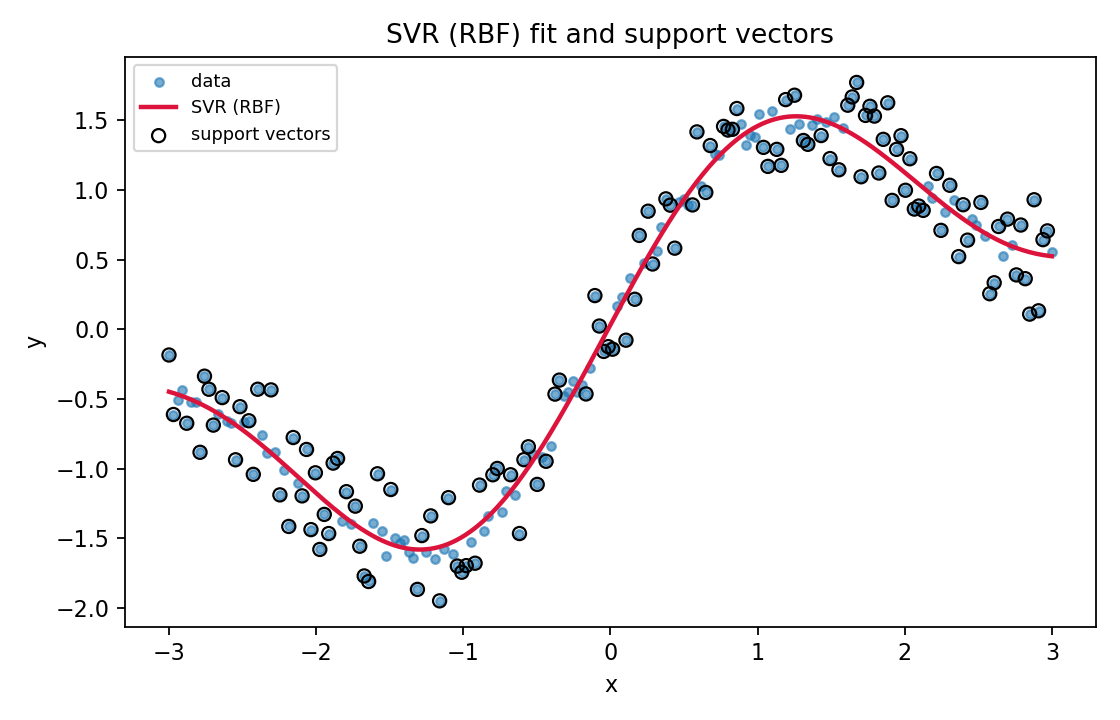
\includegraphics[width=0.85\linewidth]{svr_rbf_fit.png}
  \caption{SVR (RBF) fit and support vectors on synthetic data}
  \label{fig:svr_rbf_fit}
\end{figure}

\begin{figure}[H]
  \centering
  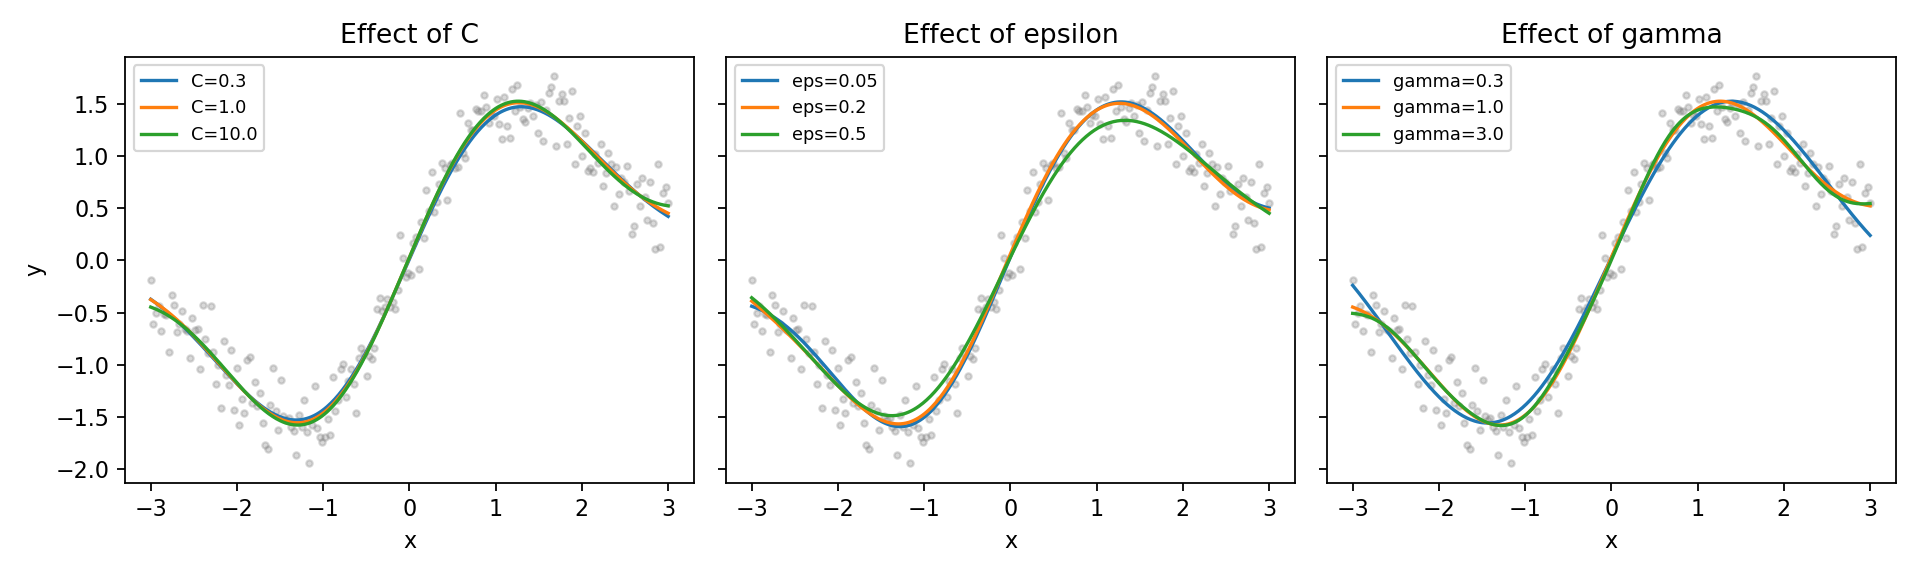
\includegraphics[width=0.95\linewidth]{svr_params_effect.png}
  \caption{Hyperparameter effects: varying \(C\), \(\varepsilon\), \(\gamma\)}
  \label{fig:svr_params}
\end{figure}

\FloatBarrier

\section{Summary}
SVR combines margin-based regularization with \(\varepsilon\)-insensitive loss and kernels to model non-linear relationships robustly. Standardization and cross-validated tuning of \(C,\varepsilon,\gamma\) are essential for reliable performance.

\end{document}

